\section{Einleitung}
\label{sec:Einleitung}

Ziel dieses Versuches ist es, die effektive Masse der Leitungselektronen in n-dotiertem
Galliumarsenid (GaAs) zu bestimmen. Dafür wird der Faraday-Effekt ausgenutzt und eine Vergleichsmessung
zwischen reinem und dotiertem GaAs durchgeführt, um den Effekt der Leitungselektronen zu isolieren.

\section{Theorie}
\label{sec:Theorie}

Für diesen Versuch wird Galliumarsenid verwendet, es handelt sich dabei um einen Halbleiterwerkstoff.
GaAs kann undotiert oder dotiert vorkommen, von besonderem Interesse für diesen Versuch sind dotierte
Varianten, da diese Leitungselektronen aufweisen. Allgemein zeichnen sich Halbleiter
dadurch aus, dass sie über diese Elektronen verfügen, die durch Anregung leicht ins Leitungsband springen
können und somit eine elektrische Leitfähigkeit generieren. Diesen Leitungselektronen lässt sich
eine effektive Masse zuordnen, welche in diesem Versuch bestimmt werden soll und im nächsten Kapitel
näher erläutert wird.

\subsection{Effektive Masse}

Zum Verständniss der effektiven Masse bietet es sich an, die Bandstruktur eines Halbleiters im k-Raum
zu betrachten. Diese ist in \autoref{fig:Halbleiter} graphisch dargestellt.

\begin{figure} [H]
    \centering
    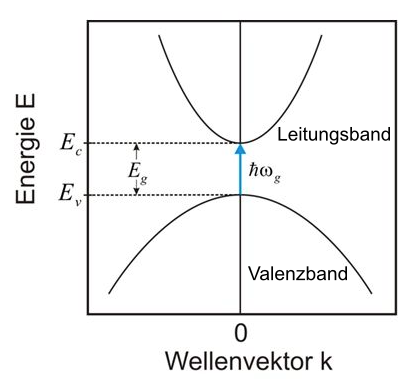
\includegraphics[height=8cm]{content/Halbleiter.png}
    \caption{Bandstruktur eines Halbleiters im k-Raum. \cite{Halbleiter}}
    \label{fig:Halbleiter}
\end{figure}

Die Bandstruktur weißt einen nahezu parabelförmigen Verlauf auf, weshalb sich eine Taylorentwicklung der unteren Kante des
Leitungsbandes bis zur zweiten Ordnung anbietet:

\begin{equation}
    E(\vec{k})=E\left(0\right)+\frac{1}{2}\sum_{i=1}^3\left(\frac{\partial E^2}{\partial k_i^2}\right)_{k=0}k_i^2+...\,
    \notag
\end{equation}
 
Vergleicht man dies mit einem harmonischen Oszillator mit

\begin{equation}
    E=\frac{\hbar k^2}{2m}\,
    \notag
\end{equation}

so fällt auf, dass sich der zweite Koeffizient der Taylorentwicklung als effektive Masse $m_i^*$ interpretieren lässt:
    
\begin{equation}
    m_i^*:=\frac{\hbar^2}{\left(\frac{\partial\epsilon^2}{\partial k_i^2}\right)_{k=0}}\,
    \notag
\end{equation}

Unter der Annahme, dass der Kristall in alle Richtungen nahezu symmetrisch ist, kann eine allgemeine effektive Masse
$m^*$ definiert werden, die sich eignet, um die Dynamik der Leitungselektronen zu beschreiben. Im wesentlichen
lassen sich die Leitungselektronen somit als freie Elektronen beschreiben, deren Wechselwirkung mit dem Kristallgitter
über die veränderte Masse $m^*$ beschrieben wird.

\subsection{Zirkulare Doppelbrechung und Faraday Effekt}
\label{sec:Faraday}

In optisch aktiven Medien kann zirkuläre Doppelbrechung auftreten. Diese beschreibt die
Fähigkeit eines Kristalles, die Polarisationsebene eines linear polarisierten Lichtstrahles bei der Transmission zu drehen.
Die Ursache liegt dabei darin, dass Phasengeschwindigkeiten für links- und rechtszirkular polarisiertes Licht in dem Kristallmedium verschieden sind.
Hierbei kann linear polarisiertes Licht als Überlagerung von links- und rechtszirkular polarisiertes Licht verstanden werden, sodass
beim Durchqueren des Mediums aufgrund der unterschiedlichen Geschwindigkeiten eine Rotation der Polarisationsrichtung stattfindet. \cite{V46Anhang}

Durch anlegen eines B-Feldes parallel zur Ausbreitungsrichtung des Lichtes kann in optisch inaktiven Medien die selbe Rotation erzeugt werden, dies
wird auch als Faraday Effekt beschrieben. Der physikalische Hintergrund ist hierbei, dass die Leitungselektronen durch das Magnetfeld auf Kreisbahnen
gezwungen werden. Es lässt sich eine Formel herleiten, die die Rotation der Polarisationsebene in Abhängigkeit der Wellenlänge angibt:

\begin{equation}
    \theta(\lambda)=\frac{\text{e}_0^3}{8\pi^2\epsilon_0c^3}\frac{1}{{m^*}^2}\frac{NBL}{n}\lambda^2\,
    \label{eq:theta}
\end{equation}

Sind alle vorkommenden Größen bekannt, also das Magnetfeld $B$, die Ladungsträgerdichte $n$ und die Länge der Probe $L$, kann die effektive Masse
$m^*$ durch umstellen von \eqref{eq:theta} berechnet werden.
Aus praktischen Gründen wird mit $\theta_\text{frei}$ gerechnet, hier wird der Rotationswinkel $\theta$ auf die Länge der Probe normiert, indem dadurch
geteilt wird.